\documentclass[11pt]{article}

\usepackage[spanish,activeacute]{babel}
\usepackage{titlesec}
\usepackage{graphicx}
\usepackage{float}
\usepackage[bottom]{footmisc}
\usepackage[hidelinks]{hyperref}
\usepackage{subcaption}
\usepackage[most]{tcolorbox}
\usepackage{xcolor}
\usepackage{enumitem}


\setlength{\parindent}{1.0em}
\setlength{\parskip}{1.0em}
\setlength{\emergencystretch}{5.0em}
\setlength{\belowcaptionskip}{-10pt}
\counterwithin{figure}{section}
\titlespacing*{\section}{0em}{3.5em}{1.5em}
\setcounter{tocdepth}{2}
\hypersetup{
	linktoc=all
}
\setlist[itemize]{topsep=0cm}


\title{\Huge Backups}
\author{Eugenia Damonte, Ariel Fideleff y Mart\'in Go\~ni}
\date{}


\definecolor{light-orange}{RGB}{168,87,0}
\definecolor{light-blue}{RGB}{64, 76, 201}
\definecolor{dark-gray}{RGB}{100,100,100}
\definecolor{light-red}{RGB}{201, 60, 60}
\definecolor{fuchsia}{RGB}{168,0,168}


\newtcolorbox{code-box}{colback=white!75!gray,colframe=white!15!gray,fontupper=\linespread{1.15}\selectfont}


\newcommand{\imagecaption}[1]{\vspace{-7pt}\caption*{\char91\ref{fig:#1}\char93}}
\newcommand{\codetext}[2]{\large\texttt{\textcolor{#1}{#2}}}
\newcommand{\rsync}[0]{\textbf{rsync}}
\newcommand{\backup}[0]{\texttt{Backup}}
\newcommand{\customitem}[1]{\item \textbf{#1:}}


\begin{document}
	\pagenumbering{gobble}
	\maketitle
	\newpage
	\tableofcontents
	\newpage
	\pagenumbering{arabic}

	
	\section{Backups}
	\subsection{Que es un backup}
		En el mundo del IT un backup es una copia de parte o toda la informaci'on de una computadora, almacenada en una unidad de almacenamiento distinta a la de la computadora. Esta puede luego ser usada para recuperar la informac'on original en caso de que ocurra una p'erdida de datos. Es importante recalcar que una p'erdida de datos puede ocurrir no solo debido a daño al sistema, ya sea de hardware o software, sino que tambi'en puede ser provocada por un error humano(por ejemplo borrar un archivo importante). Para cumplir su funci'on un backup debe contener por lo menos una copia de toda la informaci'on que se considere vale la pena guardar. Esto nos introduce a un dilema muy importante, ¿que informaci'on vale la pena guardar?

		En principio uno podría pensar que simplemente deber'iamos hacer un backup de todo el sistema, para no tener que tomar esta decisi'on. Sin embargo a medida que crece el tama'no y complejidad del sistema se vuelve cada vez mas costoso, en todo sentido, realizar backups completos. Algo que tambi'en se debe tomar en cuenta al hacer esta decisi'on es el valor del sistema en s'i, es decir cuanto vale el sistema operativo, sus configuraciones y ajustes. Si bien a simple vista esto puede parecer algo no muy importante en sistemas grandes y complejos, que requieren una gran cantidad de conocimiento y experiencia para configurar la configuraci'on puede ser igual de valiosa que la informaci'on que almacena el sistema.

	 \subsection{Tipos de backups}
		Antes de poder elegir que tipo de backup hacer hay que elegir que m'etodo utilizar para el mismo, los dos que se usan hoy en d'ia son:
		\begin{itemize}
			\customitem{Backup por archivos} El backup por archivos es la forma original en que se hac'ian los backups. En este todos los archivos y carpetas a los que se les debe realizar un backup son copiados utilizando las utilidades proveídas por el sistema operativo. Este m'etodo si bien es simple tambi'en es lento y consume una gran cantidad de recursos.\footnote{Esto se debe a que para copiar un archivo utilizando el sistema operativo se debe: Encontrar los bloques en el disco duro donde se encuentra la carpeta que contiene al archivo, leer la carpeta, buscar el archivo especificado, determinar en que bloques se encuentra y finalmente copiarlo.}
			\customitem{Backup por im'agenes} Otra opci'on que esta ganando popularidad es el backup por im'agenes, este m'etodo sobrepasa gran parte de las utilitades del sistema operativo, copiando bloques del disco duro de manera directa. Esto le permite ser mucho m'as eficiente a la hora de copiar archivos que han sido modificados, esto es porque no es necesario copiar todo el archivo, solo los bloques que han sido modificados. 
		\end{itemize}

		Cabe destacar que estos m'etodos no son mutuamente exclusivos, se pueden usar en conjunto para obtener mayor eficiencia y robustez. Por ejemplo se puede tener un sistema que haga un backup por im'agen diariamente y uno por archivos semanalmente.

		Una vez que se decidi'o que metodo utilizar para hacer los backups ahora hay que decidir que m'etodo usar para los mismos. Los backups se dividen en tres tipos:
		\begin{itemize}
			\customitem{Backup completo} Es el mas simple y el m'etodo original que se usaba para hacer los backups. Copia toda la informaci'on en el sistema especificado. Lo bueno de este m'etodo es que el backup es autocontenido, esto significa que no se requiere de ning'un otro tipo de informaci'on o archivo para que este funcione. Por el otro lado, se necesitan grandes cantidades de espacio y pueden ser casi id'enticos a backups completos anteriores.
			\customitem{Backup diferencial} Este tipo de backup solo copia las diferencias entre el sistema actual y el del 'ultimo backup completo. La principal ventaja de este m'etodo es que es mucho mas r'apido y ocupa mucho menos espacio que un backup completo. La desventaja es que para poder recupera la informaci'n con un sistema de backup diferencial se necesita el 'ultim backup completo junto con el backup diferencial.
			\customitem{Backup incremental}El backup incremental solo copia diferencias entre el el sistema actual y el 'ultimo backup completo, diferencial o incremental. La ventaja es que es a'un mas r'apido y ocupa menos espacio que un backup diferencial. El gran inconveniente con esta forma de backup es que para recuperar la informaci'on se necesitan todos los backups incrementales anteriores junto con el 'ultimo backup completo. Debido a esto recuperar informaci'on con este tipo de sistema puede ser un proceso largo.
		\end{itemize}


	\section{rsync}
	\subsection{Que es rsync}
		%The empty statement after "\rsync" is because LaTeX ignores spaces after macros, an empty statement is used to break it. Refer to: https://tex.stackexchange.com/questions/31091/space-after-latex-commands
		\rsync{} es una utilidad que permite transferir y sincronizar archivos, entre otras cosas, entre una computadora y un disco duro. Tambi'en es capaz de realizar esta tareas usando dispositivos de red. Su uso es muy com'un en sistemas basados en Unix, dada su simplicidad y facilidad de uso.

		El programa inicial fue escrito por Andrew Tridgell y Paul Mackerras, en C. Su primera versi'on se anunci'o en Junio de 1996, luego en 1999 Tridgell habl'o sobre el diseño y la implementaci'on de \rsync{} en su tesis. Es similar a la utilidad \texttt{rdist -c} creada por Ralph Campbell en 1983. Actualmente Wayne Davison se encarga de mantener el proyecto

	\subsection{Instalaci'on de rsync}
		Antes de poder usar \rsync{} tuvimos que instalarlo. Si bien hoy en d'ia suele venir incluido con la gran mayor'ia de las distros, debido a que Debian 7 es bastante viejo no la incluye. Para instalarlo usamos el comando \texttt{sudo apt-get install rsync}.

		\begin{figure}[H]
    			\centering
    			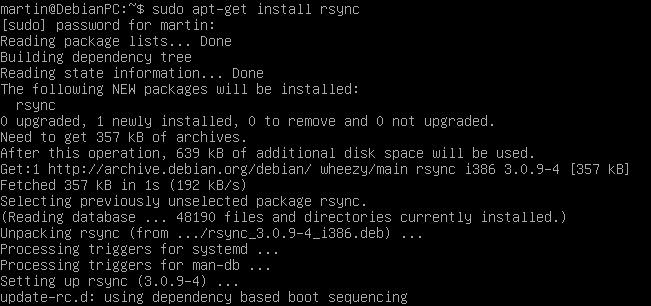
\includegraphics[scale=0.7]{Images/rsync/rsync_install.PNG}
    			\caption{Instalamos \rsync{} con \texttt{sudo apt-get install rsync}.}
    			\label{fig:rsync_install}
		\end{figure}

	\subsection{Uso b'asico de rsync}
	\subsubsection{Preparando el disco}
		Lo primero que necesitamos para hacer un backup de cualquier tipo es una unidad de almacenamiento para guardar el backup. En nuestro caso simplemente creamos otro disco duro y lo ``conectamos'' a la VM. Para hacer esto con la m'aquina apagada abrimos la configuraci'on y fuimos a \texttt{Storage}. All'i apretamos el bot'on para a'nadir un disco duro, esto nos llevo a un men'u  dond elegimos crear un nuevo disco. Especificamos el tipo y tama'no del disco y presionamos \texttt{Create}. Finalmente montamos el disco, para esto volvimos a apretar el bot'on para a'nadir una disco duro y seleccionamos el creado.

		Es importante destacar que no se debe usar un pen drive para realizar backups. Esto es porque los transistores que almacenan informaci'on en los mismos no est'an hechos para soportar el n'umero de escrituras que se necesitan para una unidad de backup. Esto a largo plazo causa que algunos de los transistores en ellos se queden ``trabados''\footnote{Realmene no se quedan ``trabados'' sino que el transistor, normalmente un FGT, pierde su capacidad de cargarse y descargarse, y por tanto de cambiar de estado.} en una posici'on haciendo imposible contiunar us'andolo. Con el tiempo esto causa deteriorio en la capacidad y velocidad de funcionamiento de la unidad y puede incluso causar perdida de datos.

		\begin{figure}[H]
    			\centering
    			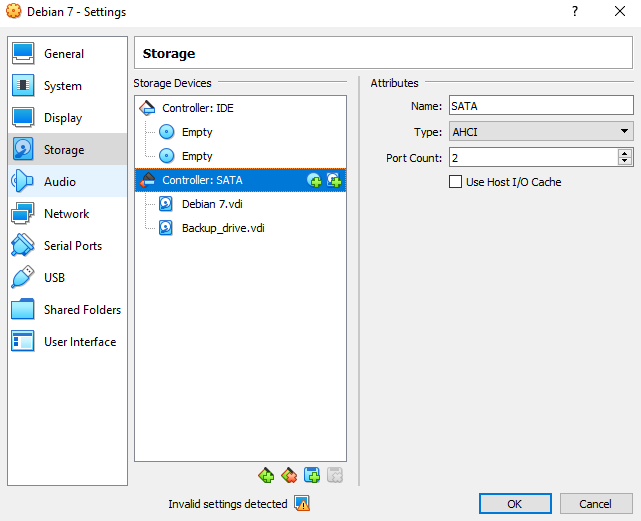
\includegraphics[scale=0.65]{Images/rsync/rsync_hdd_config.PNG}
    			\caption{Creamos un nuevo disco y lo montamos en la VM}
    			\label{fig:rsync_hdd_config}
		\end{figure}

		Ahora que nuestra VM pod'ia ver el disco hab'ia que montarlo y configurarlo. Primero utlizamos el comando \texttt{sudo fdsik -l} para verificar que el disco fuese detectado por el sistema. Al usar el comando este nos mostr'o que había un disco llamado \texttt{/dev/sdb} de 10GB, ese era el disco que hab'iamos montado.

		\begin{figure}[H]
    			\centering
    			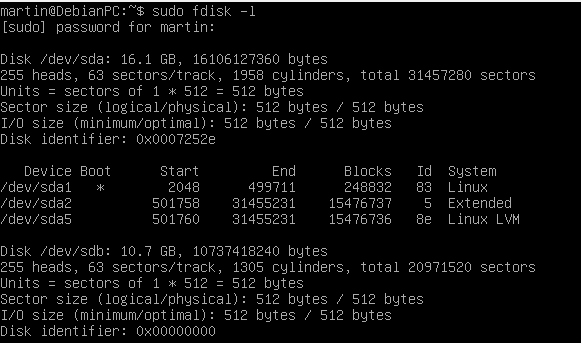
\includegraphics[scale=0.55]{Images/rsync/rsync_disk_info.PNG}
    			\caption{Usamos el comando \texttt{sudo fdsik -l} para verificar que el disco fuese detectado por el sistema.}
    			\label{fig:rsync_disk_info}
		\end{figure}

		Sabiendo el nombre del disco procedimos a particionarlo y formatearlo. Para esto usamos el comando \texttt{sudo cfdisk /dev/sdb}, este abri'o \texttt{cfdisk} una utilidad que permite crear particiones de discos. Primero nos aseguramos de que este fuese el disco que hab'iamos montado y no solo uno con esa capacidad mirando el tipo de sistema de archivos, este decia \texttt{Free Space}, es decir que no estaba formateado, era nuestro disco. Entonces seleccionamos la opci'on \texttt{New} para crear una nueva partici'on, dejamos el tama'no especificado por \texttt{cfdisk}, que es el m'aximo que permite la unidad. Esto nos devolvi'o al men'u principal, para confirmar los cambios usamos la opci'on \texttt{Write} para escribir los cambios a la tabla de discos del sistema. 

		\begin{figure}[H]
    			\centering
    			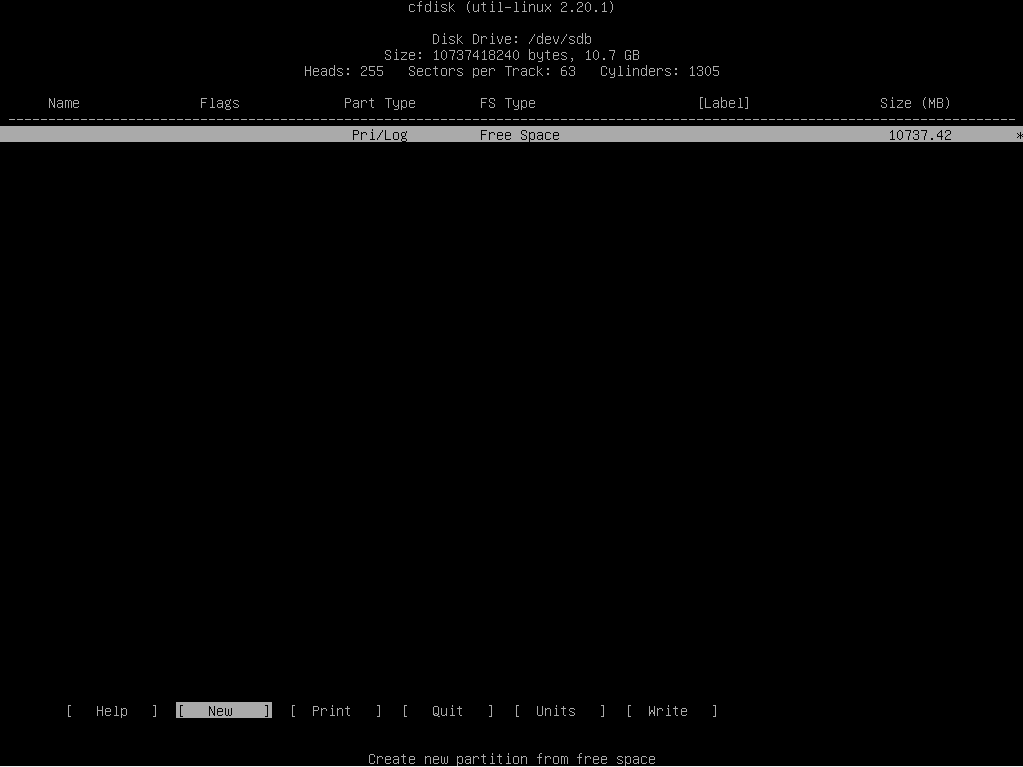
\includegraphics[scale=0.40]{Images/rsync/rsync_disk_partition.PNG}
    			\caption{Usamos \texttt{cfdisk} para crear una partici'on en el disco nuevo.}
    			\label{fig:rsync_disk_partition}
		\end{figure}

		Finalmente confirmamos que la operaci'on se hab'ia realizado de manera exitosa usando la opci'on \texttt{Print}. Esta nos mostr'o que efectivamente hab'ia una partici'on en el disco.

		\begin{figure}[H]
    			\centering
    			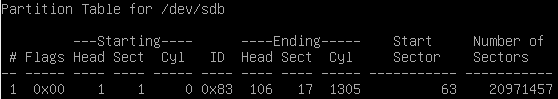
\includegraphics[scale=0.65]{Images/rsync/rsync_disk_table.PNG}
    			\caption{Una vez creada la partici'on la verificamos con la opci'on \texttt{Print}.}
    			\label{fig:rsync_disk_table}
		\end{figure}

		Ahora que ya ten'iamos una particion que pod'iamos usar llego el momento de formatearla para eso usamos el comando \texttt{sudo mkfs.ext4 /dev/deb}. Lo que hizo fue formatear el disco con el formato \texttt{ext4},\footnote{\texttt{ext4}(fourth extended filesystem) es un sistema de archivos transacional que reemplazo a ext3.} para poder as'i montarlo.
		
 		\begin{figure}[H]
    			\centering
    			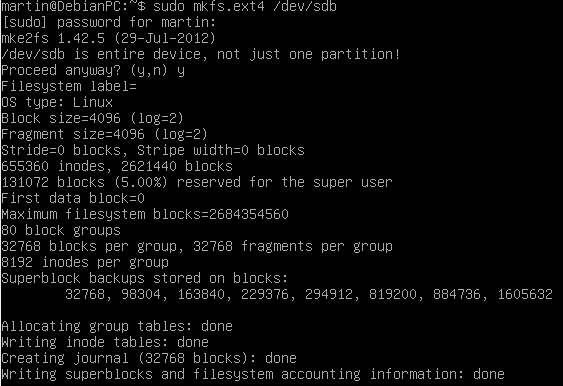
\includegraphics[scale=0.65]{Images/rsync/rsync_disk_format.PNG}
    			\caption{Formateamos el disco con el comando \texttt{sudo mkfs.ext4 /dev/deb}.}
    			\label{fig:rsync_disk_format}
		\end{figure}

		Como 'ultimo paso montamos el disco para poder usarlo. Para esto primero creamos una carpeta en la cual montar el disco, normalmente estas se encuentran en el directorio \texttt{/mnt}. Entonces creamos la carpeta \texttt{/mnt/sdb} con el comando \texttt{sudo mkdir /mnt/sdb}.

		\begin{figure}[H]
    			\centering
    			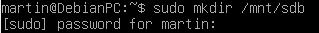
\includegraphics[scale=0.75]{Images/rsync/rsync_disk_mount.PNG}
    			\caption{Creamos el directorio donde montar el disco con \texttt{sudo mkdir /mnt/sdb}.}
    			\label{fig:rsync_disk_mount}
		\end{figure}

		Finalmente montamos el disco para poder usarlo con \texttt{sudo mount /dev/sdb /mnt/sdb}. El problema con solo hacer esto es que tendr'iamos que volver a montar el disco cada vez que iniciacemos el sistema. Para solucionar esto cambiamos el archivo \texttt{/etc/fstab}, que almacena los discos que deben ser montados al iniciar el sistema. Abr'imos el archivo para editarlo con el comando \texttt{sudo vi /etc/fstab}, luego a'nadimos lo siguiente al final del mismo:

		\begin{figure}[H]
			\centering
			\begin{code-box}
				\codetext{dark-gray}{/dev/sdb /mnt/sdb ext4 defaults 0 0}
			\end{code-box}
		\end{figure}
		
		\begin{figure}[H]
    			\centering
    			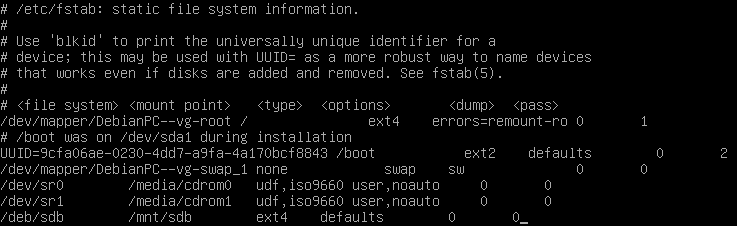
\includegraphics[scale=0.65]{Images/rsync/rsync_disk_automount.PNG}
    			\caption{Editamos \texttt{sudo vi /etc/fstab} para que el disco se monte automaticamente al iniciar la m'aquina.}
    			\label{fig:rsync_disk_automount}
		\end{figure}

		El primer elemento es el camino del disco, el segundo a donde debe ser montado y el tercero el sistema de archvios. Los dem'as los dejamos con sus valores por defecto. Hab'iendo hecho esto el disco deber'ia montarse automaticamente cada vez que iniciemos la m'aquina. Como una verificaci'on usamos el comando \texttt{mount \textbar\/ grep ``sdb''}, lo que hace es listar todos los discos montados y buscar uno llamado \texttt{``sdb''}.

		\begin{figure}[H]
    			\centering
    			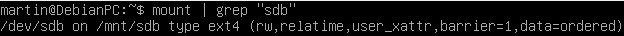
\includegraphics[scale=0.65]{Images/rsync/rsync_disk_check.PNG}
    			\caption{Verificamos que el disco este estuviese montado correctamente con \texttt{mount \textbar\/ grep ``sdb''}.}
    			\label{fig:rsync_disk_check}
		\end{figure}

		Al ejecutar el comando vimos que efectivamente hab'ia un disco montado llamado \texttt{``sdb''}, confirmando que el disco estaba montado correctamente. Ahora que el disco estaba montado y funcionando decidimos probar almacenar algo en el, solo para probar. Nos movimos a el mismo con \texttt{cd /mnt/sdb} y luego usamos el comando \texttt{touch Prueba} para intentar crear un archivo. Al ejecutar el comando el sistema nos dijo que no ten'iamos los permisos para crear un archivo. Cuando listamos los permisos del disco con \texttt{ls -l ..}, se volvio claro porque. El due'no del disco era el usuario \texttt{root}, no nuestro usuario.

		\begin{figure}[H]
    			\centering
    			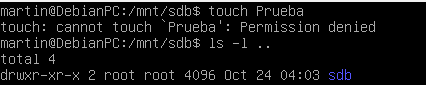
\includegraphics[scale=0.75]{Images/rsync/rsync_disk_touch.PNG}
    			\caption{Intentamos crear un archivo con \texttt{touch Prueba}.}
    			\label{fig:rsync_disk_touch}
		\end{figure}

		Para solucionar esto nos movimos a la carpeta \texttt{/mnt}(donde \texttt{sdb} se encuentra) y usamos el comando \texttt{sudo chown -R martin:martin sdb} para cambiar el due'no de la carpeta de \texttt{root} a \texttt{martin}. Habiendo hecho esto repetimos la prueba con \texttt{touch} y esta fue exitosa.

		\begin{figure}[H]
    			\centering
    			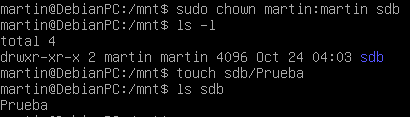
\includegraphics[scale=0.75]{Images/rsync/rsync_disk_works.PNG}
    			\caption{Cambiamos el due'no de \texttt{sdb} para solucionar el problema y lo verificamos.}
    			\label{fig:rsync_disk_works}
		\end{figure}

		Finalmente con el disco funcionando correctamente decidimos comenzar con la pr'oxima parte del trabajo, hacer backups con \rsync{} usando el nuevo disco.

	\subsubsection{Usando rsync}
		Habiendo llegado la hora de usar \rsync{} decidimos hacer un backup completo de una carpeta en nuestro directorio propio como prueba de uso. Seleccionamos la carpeta \texttt{C}, que ten'ia todo el c'odigo correspondiente a el trabajo practico sobre software en formato fuente. La elegimos porque era una carpeta que a su vez ten'ia varias sub carpetas con archivos en ellas, lo que nos permit'ia probar las opciones recursivas de \rsync{}. Antes de hacer el backup creamos la carpeta a donde los guardar'iamos, \texttt{/mnt/sdb/Backups}, lo hicimos con el comando \texttt{mkdir /mnt/sdb/Backups}.

		\begin{figure}[H]
    			\centering
    			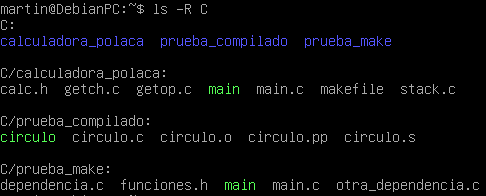
\includegraphics[scale=0.80]{Images/rsync/rsync_backup_C_contents.PNG}
    			\caption{Los contenidos del directorio \texttt{C}.}
    			\label{fig:rsync_C_contents}
		\end{figure}

		El uso b'asico de \rsync{} es bastante simple, primero se pone el directorio desde el que se quiere copiar y luego hacia cual se quiere copiar. Para empezar esto fue lo que hicimos, usamos el comando \texttt{rsync \textasciitilde/C /mnt/sdb/Backup}, al hacerlo el mensaje \textit{skipping directory C} apareci'o. Cuando revisamos los contenidos de \backup{} vimos que estaba vac'io. Esta situaci'on se explica si miramos los contenidos del directorio \texttt{C}, dentro de el solo hay carpetas, no archivos. Entonces al no encontrar archivos que copiar dentro de la carpeta especificada \rsync{} simplemente la omiti'o y no copi'o nada. Dado este problema a'nadimos la opci'on \texttt{-r} a el comando,  para copiar tamb'ien los contenidos de todas las subcarpetas. Al ejecutar el comando y luego verificar los contenidos de \backup{} vimos que ahora hab'ia una carpeta llamada \texttt{C} en ella, indicando que los archivos efectivamente se hab'ian copiado.

		\begin{figure}[H]
    			\centering
    			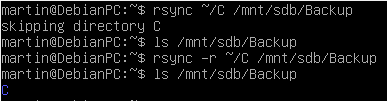
\includegraphics[scale=0.80]{Images/rsync/rsync_backup_first_try.PNG}
    			\caption{Nuestro primer intento de usar \rsync{}.}
    			\label{fig:rsync_backup_first_try}
		\end{figure}

		Para asegurarnos de que la copia hubiese efectivamente ocurrido listamos los contenidos de \backup{} con \texttt{ls -Rl /mnt/sdb/Backup}, esto nos revel'o algo interesante, todos los archivos ten'ian la fecha de modificaci'on de cuando hab'iamos realizado el backup. Esto ten'ia sentido ya que esos archivos se crearon y modificaron al momento en que nosotros realizamos el backup. Sin embargo nos preguntamos si hab'ia alguna manera de conservar la fecha original. Entonces decidimos leer las opciones de \rsync{}, para ver si se pod'ia, junto con tal vez encontrar otras opciones 'utiles.

		\begin{figure}[H]
    			\centering
    			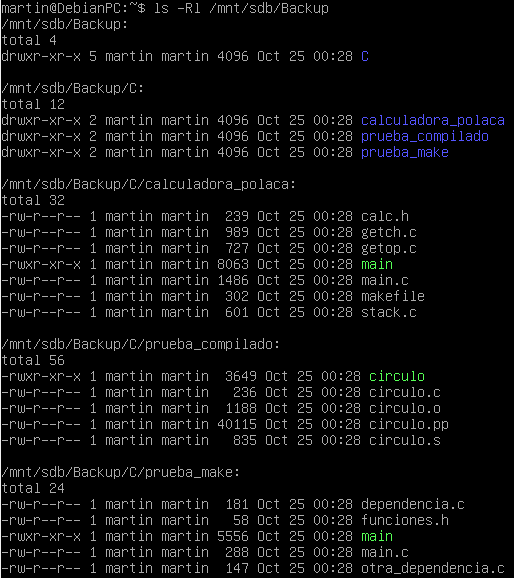
\includegraphics[scale=0.80]{Images/rsync/rsync_backup_contents.PNG}
    			\caption{Los contenidos de \backup{}, mostrados con {ls -Rl /mnt/sdb/Backup}.}
    			\label{fig:rsync_backup_contents}
		\end{figure}

		Luego de leer la p'agina de \texttt{man} de \rsync{} encontramos no solo opciones 'utiles sino tambi'en informaci'on sobre como mejor usar el comando y adaptarlo mejor a nuestras necesidades.

		Lo primero que encontramos fue una secci'on referida a el uso de la barra(\texttt{/}). Si se pone al final del directorio desde el que se quiere copiar cambia la forma en la que \rsync{} almacena los archivos copiados. Lo que hace es evitar crear un directorio adicional, copiando directamente los contenidos del directorio especificado sin el directorio en s'i. La diferencia se puede observar mejor en la figura \ref{fig:rsync_backup_forwardslash}.

		\begin{figure}[H]
    			\centering
    			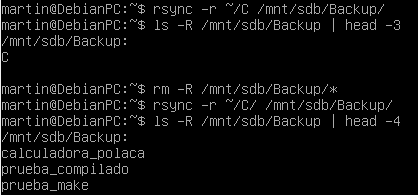
\includegraphics[scale=0.80]{Images/rsync/rsync_backup_forwardslash.PNG}
    			\caption{La diferencia entre usar y no usar la barra en \rsync{}.}
    			\label{fig:rsync_backup_forwardslash}
		\end{figure}

		En cuanto a las opciones encontramos varias que nos parecieron bastante 'utiles. La primera que probamos fue \texttt{-v}(verbose), como indica su nombre lo que hace es hacer la salida de \rsync{} mucho m'as verbosa haciendo que muestre que es lo que esta copiando asi como cuantos bytes copia y cuanto tiempo le lleva. Otra opci'on que tambi'en nos pareci'o 'util pero algo peligrosa es \texttt{--delete}. Lo que hace es eliminar cualquier archivo en el directorio de destino que no este en el directorio a copiar. La raz'on de su peligrosidad es su principio de funcionamiento, si hay algun archivo en la carpeta de destino que desamos conservar pero este no esta en la carpeta a copiar sera borrado.

		\begin{figure}[h]
			\centering
			\begin{subfigure}{0.75\linewidth}
				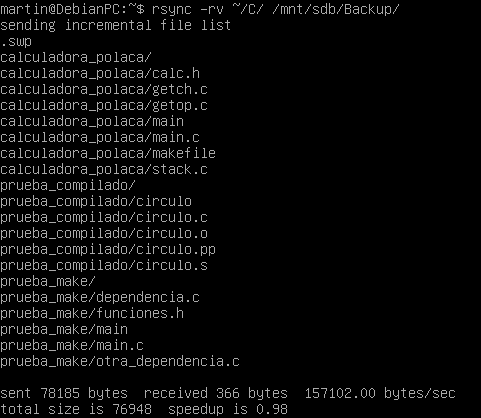
\includegraphics[width=1\linewidth]{Images/rsync/rsync_backup_verbose.PNG}
				\caption{\rsync{} con la opci'on \texttt{-v}.}
			\end{subfigure}
			\bigbreak
			\begin{subfigure}{0.7\linewidth}
				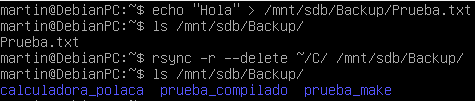
\includegraphics[width=1\linewidth]{Images/rsync/rsync_backup_delete.PNG}
				\caption{\rsync{} con la opci'on \texttt{--delete}.}
			\end{subfigure}
			\caption{Probamos usar las opciones \texttt{-v} y \texttt{--delete} con \rsync{}.}
			\label{fig:rsync_backup_options_1}
		\end{figure}

		Luego de un poco mas de b'usqueda encontramos la opci'on \texttt{-a}(archive), esta es equivalente a un gran n'umero de opciones. Es la manera de decir que uno quiere preservar casi todos los atributos sobre los archivos copiados, la unica exepci'on es que no preserva los enlaces duros.\footnote{El motivo por el que no son preservados es porque encontrar archivos que poseen m'ultiples enlaces es costoso en cuanto a recursos. Para preservarlos se debe usar la opci'on \texttt{-H}.} Las opciones a las que \texttt{-a} se expande son:

		\begin{itemize}
			\customitem{-r} Hace que el directorio a copiar se copie de manera recursiva, permitiendo copiar subdirectorios y sus contenidos.
			\customitem{-l} Mantiene los enlaces s'imbolicos encontrados.
			\customitem{-p} Mantiene los permisos originales de los archivos copiados. Sin esta opci'on los archivos existentes(incluyendo los que se actualizan) mantienen sus permisos. Para los nuevos los bits de permisos son iguales a los originales tras ser enmascarados con los bits de permiso de los predeterminados del directorio de destino.
			\customitem{-t} Hace que los tiempos de modificaci'on se transfieran de los archivos originales a los copiados. Si esta opci'on no se incluye, durante el pr'oximo backup todos los archivos van a ser actualizados, es decir copiados nuevamente.
			\customitem{-g} Mantiene el grupo de los archivos copiados. Si esta opci'on no se incluye los archivos copiados toman el grupo de el usuario que haya ejecutado el comando.
			\customitem{-o} Mantiene el due'no de los archivos copiados. Si esta opci'on no se incluye el due'no de los archivos copiados pasa a ser el usuario que haya ejecutado el comando.
			\customitem{-D} Esta opci'on se expande a dos opciones m'as, son:
			\begin{itemize}
				%"\kern" adds a non-breaking space of the specified size.
				\customitem{-{\kern 0.05em}-devices} Hace que se copien los archivos de character y bloqueo de dispositivo a el destino para recrear los dispositivos. Esta opci'on no tiene efecto si \rsync no se ejecuta como \texttt{root}.
				\customitem{-{\kern 0.05em}-specials} Hace que se copien todos los archivos especiales.
			\end{itemize}
		\end{itemize}

		Habiendo analizado las opciones de \rsync decidimos que la configuraci'on ideal, al menos en nuestro caso, ser'ia \texttt{rsync -avH ~/C/ /mnt/sdb/Backup}. Teniendo nuestra configuraci'on probamos usar el comando y funciono perfectamente, haciendo un backup de todos los elementos en el directorio \texttt{C}.

		\begin{figure}[H]
			\centering
			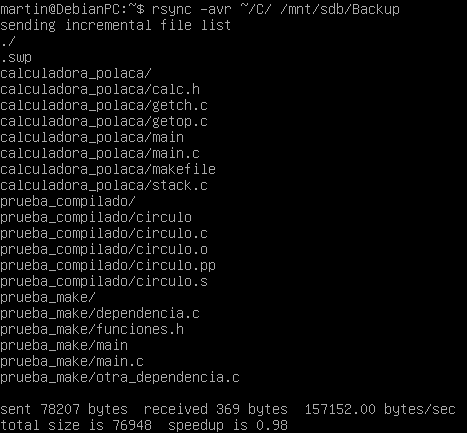
\includegraphics[scale=0.7]{Images/rsync/rsync_backup_final.PNG}
			\caption{Usamos \rsync{} con todas las opciones que decidimos.}
			\label{fig:rsync_backup_final}
		\end{figure}

		Para verificar que el backup hubiese funcionado correctamente listamos los contenidos de el \backup con el comando \texttt{ls -lr /mnt/sdb/Backup/}. Efectivamente hab'ia funcionado de manera correcta, todos los archivos estaban y ten'ian todos los atributos correctos(due'no, permisos, 'ultima modificaci'on, etc).

		\begin{figure}[H]
			\centering
			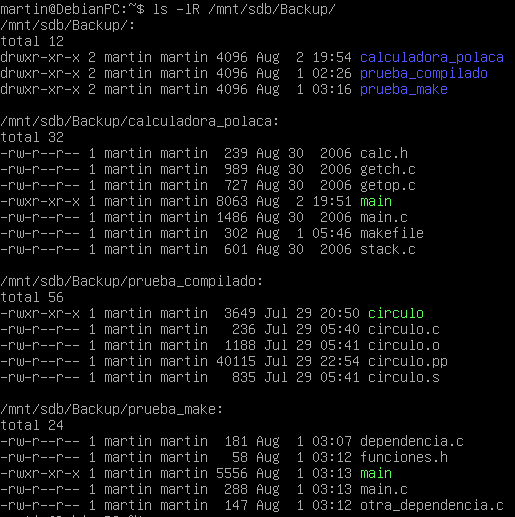
\includegraphics[scale=0.7]{Images/rsync/rsync_backup_final_result.PNG}
			\caption{Verificamos que los resultados del backup fuesen correctos.}
			\label{fig:rsync_backup_final_result}
		\end{figure}

		Como nota final creemos que vale la pena aclarar que debido nuestra configuraci'on \rsync{} hace backups incrementales,\footnote{Referirse a secci'on 1.2 - Tipos de backups.} dado que los archivos copian su fecha de modificaci'on. Por lo que si intentamos hacer un backup de la misma carpeta sin cambiar nada nign'un archivo se copiar'a.

		\begin{figure}[H]
			\centering
			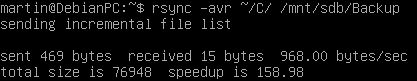
\includegraphics[scale=0.7]{Images/rsync/rsync_backup_incremental.PNG}
			\caption{Revisamos si \rsync{} hac'ia backups diferenciales con nuestra configuraci'on.}
			\label{fig:rsync_backup_incremental}
		\end{figure}


	%Looks nicer
	\newpage
	\section{Comandos usados}
		A continuaci'on se encuentran todos los comandos utilizados en este trabajo, correspondientes a las im'agenes presentadas.

		\begin{figure}[H]
			\centering
			\begin{code-box}
				\codetext{fuchsia}{sudo} \codetext{light-blue}{apt} \codetext{light-orange}{install} \codetext{light-red}{rsync}
			\end{code-box}
			\imagecaption{rsync_install}
		\end{figure}

		\begin{figure}[H]
			\centering
			\begin{code-box}
				\codetext{fuchsia}{sudo} \codetext{light-blue}{fdisk} \codetext{light-orange}{-l}
			\end{code-box}
			\imagecaption{rsync_disk_info}
		\end{figure}

		\begin{figure}[H]
			\centering
			\begin{code-box}
				\codetext{fuchsia}{sudo} \codetext{light-blue}{mkfs.ext4} \codetext{light-red}{/dev/sdb}
			\end{code-box}
			\imagecaption{rsync_disk_format}
		\end{figure}

		\begin{figure}[H]
			\centering
			\begin{code-box}
				\codetext{fuchsia}{sudo} \codetext{light-blue}{mkdir} \codetext{light-red}{/mnt/sdb}
			\end{code-box}
			\imagecaption{rsync_disk_mount}
		\end{figure}

		\begin{figure}[H]
			\centering
			\begin{code-box}
				\codetext{light-blue}{mount} \textbar{} \codetext{light-blue}{grep} \codetext{light-red}{``sdb''}
			\end{code-box}
			\imagecaption{rsync_disk_check}
		\end{figure}

		\begin{figure}[H]
			\centering
			\begin{code-box}
				\codetext{light-blue}{touch} \codetext{light-red}{Prueba}

				\codetext{light-blue}{ls} \codetext{light-orange}{-l}
			\end{code-box}
			\imagecaption{rsync_disk_touch}
		\end{figure}

		\begin{figure}[H]
			\centering
			\begin{code-box}
				\codetext{fuchsia}{sudo} \codetext{light-blue}{chown} \codetext{light-red}{martin:martin sdb}

				\codetext{light-blue}{ls} \codetext{light-orange}{-l}

				\codetext{light-blue}{touch} \codetext{light-red}{Prueba}

				\codetext{light-blue}{ls} \codetext{light-red}{sdb}
			\end{code-box}
			\imagecaption{rsync_disk_works}
		\end{figure}

		\begin{figure}[H]
			\centering
			\begin{code-box}
				\codetext{light-blue}{ls} \codetext{light-orange}{-R} \codetext{light-red}{C}
			\end{code-box}
			\imagecaption{rsync_C_contents}
		\end{figure}

		\begin{figure}[H]
			\centering
			\begin{code-box}
				\codetext{light-blue}{rsync} \codetext{light-red}{\textasciitilde/C /mnt/sdb/Backup}

				\codetext{light-blue}{ls} \codetext{light-red}{/mnt/sdb/Backup}

				\codetext{light-blue}{rsync} \codetext{light-orange}{-r} \codetext{light-red}{\textasciitilde/C /mnt/sdb/Backup}

				\codetext{light-blue}{ls} \codetext{light-red}{/mnt/sdb/Backup}
			\end{code-box}
			\imagecaption{rsync_backup_first_try}
		\end{figure}

		\begin{figure}[H]
			\centering
			\begin{code-box}
				\codetext{light-red}{ls} \codetext{light-orange}{-Rl} \codetext{light-red}{/mnt/sdb/Backup}
			\end{code-box}
			\imagecaption{rsync_backup_contents}
		\end{figure}

		\begin{figure}[H]
			\centering
			\begin{code-box}
				\codetext{light-blue}{rsync} \codetext{light-orange}{-r} \codetext{light-red}{\textasciitilde/C /mnt/sdb/Backup/}

				\codetext{light-blue}{ls} \codetext{light-orange}{-R} \codetext{light-red}{/mnt/sdb/Backup} \textbar{} \codetext{light-blue}{head} \codetext{light-orange}{-3}

				\codetext{light-blue}{rm} \codetext{light-orange}{-R} \codetext{light-red}{/mnt/sdb/Backup/*}

				\codetext{light-blue}{rsync} \codetext{light-orange}{-r} \codetext{light-red}{\textasciitilde/C/ /mnt/sdb/Backup/}

				\codetext{light-blue}{ls} \codetext{light-orange}{-R} \codetext{light-red}{/mnt/sdb/Backup} \textbar{} \codetext{light-blue}{head} \codetext{light-orange}{-4}
			\end{code-box}
			\imagecaption{rsync_backup_forwardslash}
		\end{figure}

		\begin{figure}[H]
			\centering
			\begin{code-box}
				\codetext{light-blue}{rsync} \codetext{light-orange}{-rv} \codetext{light-red}{\textasciitilde/C/ /mnt/sdb/Backup/}

				\codetext{light-blue}{echo} \codetext{light-red}{``Hola''} \textgreater{} \codetext{light-red}{/mnt/sdb/Backup/Prueba.txt}
				
				\codetext{light-blue}{ls} \codetext{light-red}{/mnt/sdn/Backup}

				\codetext{light-blue}{rsync} \codetext{light-orange}{-r --delete} \codetext{light-red}{\textasciitilde/C/ /mnt/sdb/Backup/}

				\codetext{light-blue}{ls} \codetext{light-red}{/mnt/sdn/Backup}
			\end{code-box}
			\imagecaption{rsync_backup_options_1}
		\end{figure}

		\begin{figure}[H]
			\centering
			\begin{code-box}
				\codetext{light-blue}{rsync} \codetext{light-orange}{-avr} \codetext{light-red}{\textasciitilde/C /mnt/sdb/Backup}
			\end{code-box}
			\imagecaption{rsync_backup_final}
		\end{figure}

		\begin{figure}[H]
			\centering
			\begin{code-box}
				\codetext{light-blue}{ls} \codetext{light-orange}{-lR} \codetext{light-red}{/mnt/sdb/Backup}
			\end{code-box}
			\imagecaption{rsync_backup_final_result}
		\end{figure}

		\begin{figure}[H]
			\centering
			\begin{code-box}
				\codetext{light-blue}{rsync} \codetext{light-orange}{-avr} \codetext{light-red}{\textasciitilde/C /mnt/sdb/Backup}
			\end{code-box}
			\imagecaption{rsync_backup_incremental}
		\end{figure}

\end{document}


